\section{Background and Motivation} \label{sec:motivation}

%In this section, we discuss the key weaknesses of the state-of-the-art function merging, called {\SOAName}~\cite{rocha20}, addressed in this paper.
%First, we show how different stages in {\SOAName} impact its running time.
%\textbf{TODO: Memory usage.}

%In this section, we will discuss how different stages of the state-of-the-art function merging impact during compilation time.
%present how different stages of the state-of-the-art function merging impact its running time.
%In this section, we will present how sequence alignment can be an important source of compilation time overhead.
%Then we discuss how we can address this issue by doing less work, while still keeping most of the code size reduction from the state-of-the-art technique.

In this section, we first introduce the working mechanism of \SOAName~\cite{rocha20}, the state-of-the-art function merging technique. We highlight the main drawbacks of \SOAName in terms of compile time and memory footprint. We then outline how we can address these drawbacks without compromising on the code size reduction. 

\subsection{Function Merging Based on Sequence Alignment}
Regardless of the approach, merging two functions requires identifying similar code segments in the two functions that can be profitably merged.
To do so, \SOAName first transforms each function into a linear sequence of labels and instructions. It then applies a sequence alignment algorithm to search for the optimal way to align two input sequences based on their matching subsequences. The goal of the search technique is to identify the mergeable code. In the final step, it uses the resulting aligned sequence to directly generate code.

\SOAName uses a similarity ranking strategy based on the \textit{fingerprint} of functions to determine merging candidates.  The fingerprint is a fixed-size vector that summarizes the content of the function in terms of LLVM opcodes. The fingerprint representation allows the compiler to compare functions using a simple distance metric, such as the Manhattan distance. For a given reference function, all other functions are ranked based on the distance of their fingerprints. The closest function is chosen as a merging candidate. \fixme{MC: should this paragraph also mention the outer loop? It currently sounds like you just try the best candidate.}

After merging functions, \SOAName applies a dedicated pass to repair issues arising in the single static assignment (SSA) form due to function merging. This pass is referred to as \emph{SSA fix}. It then applies a post-generator step, called \emph{Simplification}, to remove redundant instructions introduced by function merging. \fixme{PP: Both here and in Figure 1, perhaps we can merge CodeGen, Fix, and Simplification into an expanded CodeGen stage. Do we get any information from being detailed?}

%\SOAName has a search strategy for pairing similar functions for merging but avoiding a prohibitively expensive quadratic number of merging attempts.
%The purpose of the search strategy is to avoid a quadratic exploration that attempts to merge all possible pairs of functions.
%All three techniques use a ranking strategy based on the \textit{fingerprint} of the functions to evaluate their similarity.
%They start by precomputing and caching fingerprints for all functions.
%The fingerprint is a fixed-size vector that summarizes the content of the function.
%To this end, the fingerprint consists of a map of instruction opcodes to their frequency in the function.
%While functions can have several thousands of instructions, an IR usually has just a few tens of opcodes, e.g., the LLVM IR has only about 68 different opcodes.

%The fingerprint representation allows us to compare functions using a simple distance metric, such as the Manhattan distance.
%For a given reference function, all other functions are ranked based on the distance of their fingerprints.
%The candidate function with the smallest distance will be used for a merging attempt.

\subsection{Limitations of The State of The Art}

\fixme{PP: Needs some reorganisation. Either move our example at the end, after we've framed what the problem is, or make changes to the second paragraph to flow directly from the first instead of moving a step backward to discuss sequence alignment as a concept (instead of as a problem)}

When reproducing the experiments \fixme{MC: make it clear that these are SalSSA's published experiments} on our machine of 16 GB of memory, we were unable to build \texttt{602.gcc\_s}, from SPEC 2017, due to an out of memory crash.
We could only build this benchmark after migrating to a bigger machine, with 64~GB of available memory, because overall it needs over 32~GB of memory.
After investigating it further, we realized that this is due to the quadratic algorithm used for aligning two functions selected for merging.

 The main innovation of \SOAName and its predecessor is their use of an optimal sequence alignment algorithm, called the \NW algorithm, for identifying similar code segments.
 This allows it to merge arbitrary pairs of functions.
 However, the space and time complexity of this algorithm is quadratic on the size of the input sequences \cite{needleman70,carrillo88}. Because \SOAName applies the algorithm on the linearized sequences of the whole input functions, alignment brings the compilation process to a crawl for large functions. For the same reason, \SOAName also incurs a high memory footprint when merging even medium sized functions. It is impossible to compile larger ones on most workstations or even many servers, limiting {\SOAName}'s practicality.

\subsection{Compilation Overhead Breakdown} \label{sec:motivation:breakdown}

%When merging two functions, the goal is to identify which segments of the code are different and which ones are equivalent, and therefore mergeable.
%To this end, SalSSA uses an optimal sequence alignment algorithm, called the Needleman-Wunsch algorithm, which is quadratic on the size of the input sequences.
%Since SalSSA applies it on the linearised sequences of the whole input functions, the time spend aligning sequences can be significant for programs with very large functions.

\begin{figure}[t!]
  \centering
  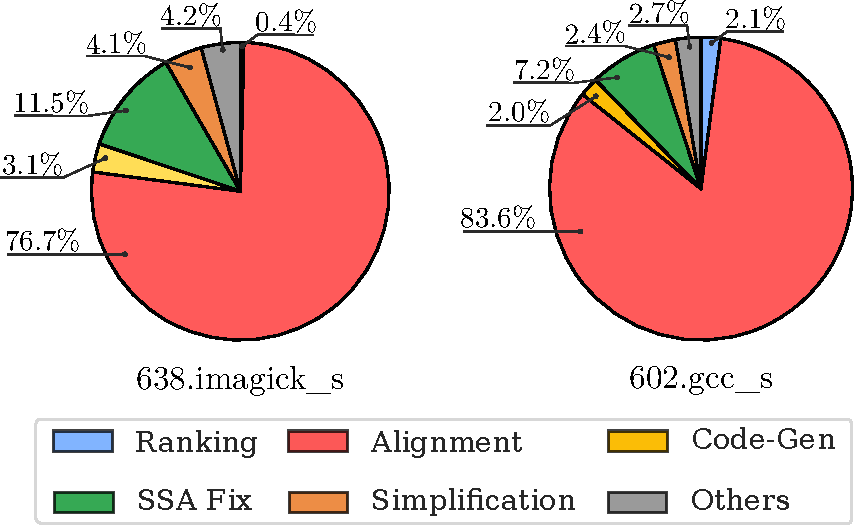
\includegraphics[width=0.85\linewidth]{figs/compilation-breakdown-motivation-alignment.pdf}
  \caption{Breakdown of the running time for the different stages of the function merging pass. Sequence alignment alone takes 25 seconds and 4.2 minutes on \texttt{638.imagick\_s} and \texttt{602.gcc\_s}, respectively.}
  \label{fig:compilation-breakdown-motivation-alignment}
\end{figure}

Figure~\ref{fig:compilation-breakdown-motivation-alignment} shows the running time breakdown for the different stages of the function merging pass in the LLVM-based \SOAName  implementation for two SPEC CPU2017 benchmarks. 
As seen in the diagram, sequence alignment dominates the running time of function merging, representing up to 83\% of its overall running time. 
Sequence alignment alone takes 25 seconds and 4.2 minutes on \texttt{638.imagick\_s} and \texttt{602.gcc\_s}, respectively.
The sequence alignment stage also causes the peak in memory usage for these two programs, 4.5~GB for \texttt{638.imagick\_s} and 32~GB for \texttt{602.gcc\_s}.
This is not surprising, as the Needleman-Wunsch algorithm has a quadratic complexity in both time and memory usage.
Because this algorithm is applied on linearized sequences of the whole input functions, programs containing large functions, such as \texttt{638.imagick\_s} and \texttt{602.gcc\_s}, are heavily affected.
%For example, \texttt{638.imagick\_s} has a total of 15,454 functions with the largest one having 73,127 instructions.
%Meanwhile, even though \texttt{602.gcc\_s} has only 2,457 functions, its largest function has 28,974 instructions; hence \SOAName also incurs significant peak memory usage when processing this program. 

Most of the rest of the running time of function merging is associated with producing merged functions from the aligned sequences. \fixme{PP: Same suggestion as earlier about CodeGen.} This includes the time spent on the code generation stage (Code-Gen), SSA reconstruction (SSA Fix), and code simplification (Simplification). These stages account for 18.7\% of the \SOAName’s running time on \texttt{638.imagick\_s} and 11.6\% on \texttt{602.gcc\_s}. Not all of this overhead contributes to code size reduction. Most of it is wasted on merged functions that will be rejected by the profitability analysis. \fixme{PP: We have not discussed profitability analysis before or that we need to merge functions before we reject them. We could add a bit more detail. Otherwise, we might want to restrict the motivation to reducing alignment overheads.}
%Because a majority of the merging attempts are unprofitable, these costs become significant for large programs.
A better approach would try to bail out from the merging process of unprofitable functions as early as possible to reduce the compilation time. 

\subsection{When Less is More}

We observe that most of the benefit of function merging often comes from merging highly similar, but not necessarily identical, basic blocks. Figure~\ref{fig:xalan-example} shows one such example extracted from the \texttt{483.xalancbmk} benchmark found in SPEC CPU2006.
This example shows the two input functions annotated with the alignment produced by \SOAName. Merging these two functions alone ends up reducing the final object file by 33 bytes. 

\begin{figure}[t]
  \centering
  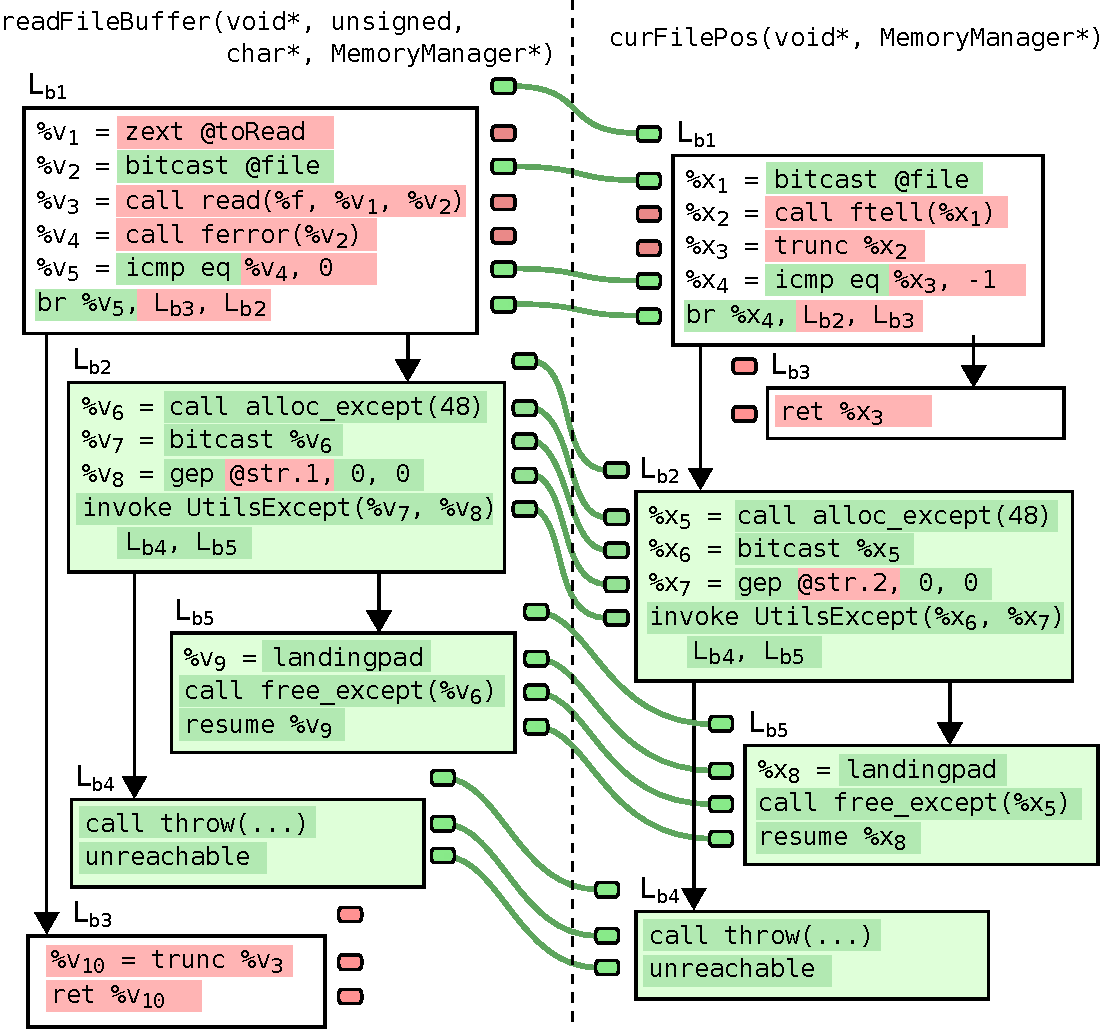
\includegraphics[width=\linewidth]{figs/xalan-example.pdf}
  \caption{Example extracted from \texttt{483.xalancbmk} found in SPEC CPU2006.}
  \label{fig:xalan-example}
\end{figure}

% \begin{figure*}[h]
%   \centering
%   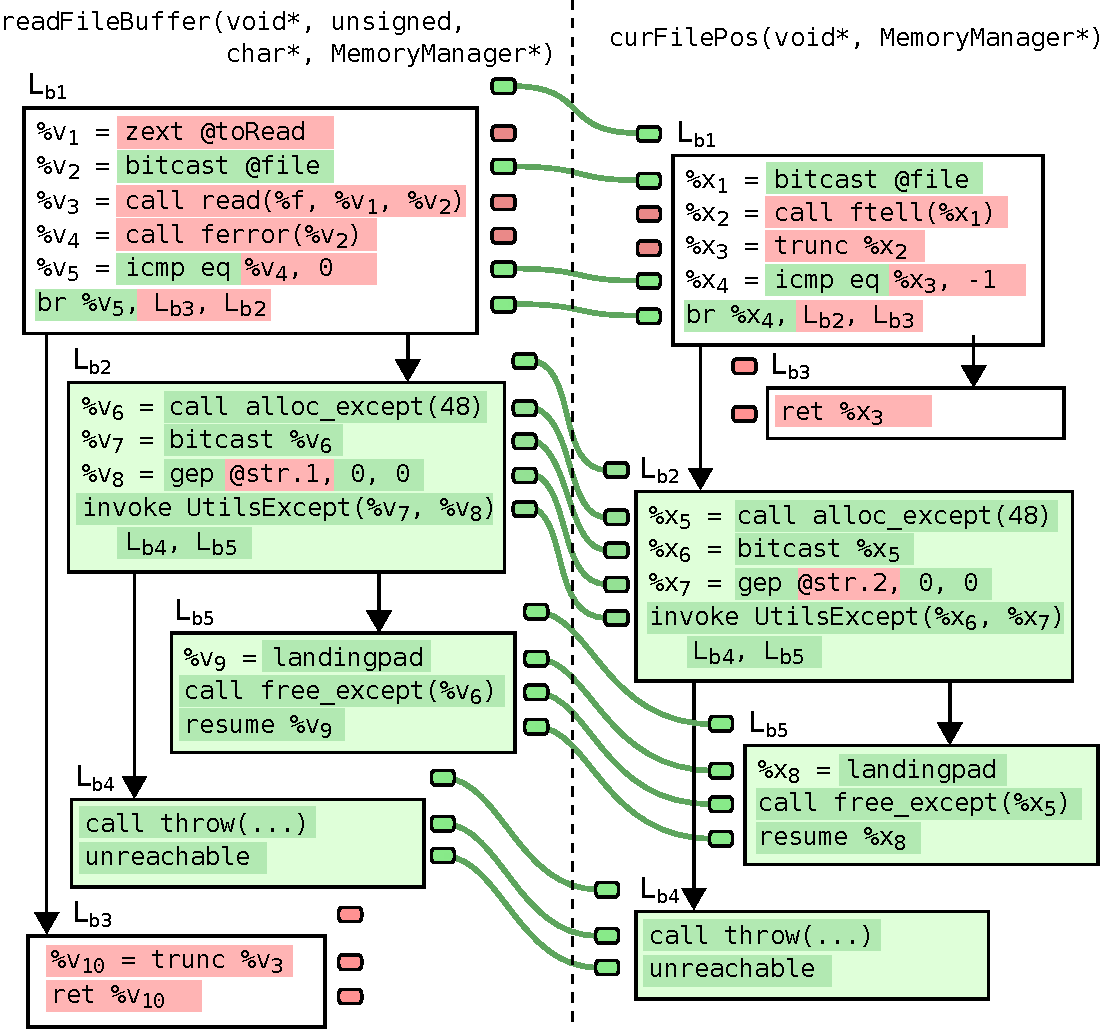
\includegraphics[width=0.6\textwidth]{figs/xalan-example.pdf}
%   \caption{Example extracted from \texttt{483.xalancbmk} found in SPEC CPU2006.}
%   \label{fig:xalan-example}
% \end{figure*}

%This example also suggests that 
While this approach is flexible enough to identify very complex alignments, what it actually produces is three aligned pairs of basic blocks and a few instructions in the entry blocks. More importantly, these entry block instructions offer nothing in terms of code size reduction. The gains of merging them are negated by the extra branches and operand selections needed to preserve the program's semantics. Since {\SOAName} analyzes the profitability of the final merged function as a whole, this unprofitable sequence of instructions will be merged because of the three highly profitable basic blocks. For the same reason, we can have profitable areas of code rejected because the rest of the merged function, as a whole, is unprofitable.


%Since {\SOAName} analyzes the profitability of the final merged function as a whole, we may have segments of unprofitably merged code inside an otherwise profitably merged function.
%Similarly, we may also have segments of profitably merged code inside merged functions that are thrown away by the profitability analysis. 
%However, we can achieve the same code size reduction of 33 bytes by merging only the subset of nearly identical basic blocks (highlighted in Figure~\ref{fig:xalan-example}).
%The gains of merging the entry blocks are negated by the extra branches and operand selections needed to preserve the program's semantics.

This example shows us that we could achieve similar code size reduction by reducing the problem of aligning functions into two simpler processes: first identifying highly similar basic blocks and then aligning the instructions in each pair of similar blocks. 
%merging functions on the basic block rather than on the instruction level adopted by \SOAName.
By operating on basic blocks, we could greatly reduce the length of the sequences to be aligned and the associated compilation and memory overhead. Furthermore, by making profitability decisions for each pair of basic blocks separately, we could avoid merging unprofitable pairs. The rest of this paper shows how we use such an approach to overcome the weaknesses of \SOAName and make function merging practical for optimizing large programs. 

%Therefore, the main takeaways are:
%1) It often suffices to merge functions on a per basic block manner. %, since crossing the basic block boundary is rarely necessary.
%2) A fine-grain profitability analysis is needed to avoid  merging unprofitable pairs of basic blocks.



%This happens because the optimal sequence alignment algorithm used by SalSSA is trying to maximize the number of matching entries, which does not necessarily translate to the optimal merged function.
%Moreover, SalSSA is also limited by the fixed linearization strategy.
%For example, the two \textit{return} instructions are not aligned due to the ordering of the basic blocks chosen by the linearization strategy.

%We can take advantage of this insight in order to design a faster function merging technique.
%Ultimately, our goal is to be able to avoid the quadratic algorithm while still producing significant reductions to the program's size.

%In this paper, we take advantage of these key insights to propose a novel function merging technique that addresses the major overheads discussed in Section~\ref{sec:motivation:breakdown}.
%We can take advantage of this insight in order to design a better and faster function merging technique.
%To this end, we propose a novel function merging technique that work on the level of basic blocks and includes a fine-grain profitability analysis.



%bail out early from   of a fine-grain and a coarse-grain analysis.

%TODO: [Relatedwork] Note that this is different from the work done by von Koch~et~al.~\cite{edler14}, as these two functions are not \textit{structurally similar} as expected by their function merging technique and therefore could not be merged.
